\subsection{Evaluation}

Questgram has undergone a two-fold evaluation, %was evaluated through a dynamic analysis experiment and user-study. This decision is based on Shaker et al. argues that a hybrid approach with both a 
top down (expressivity analysis) and bottom up (user study), as suggested by Shaker et al \citepeighth{p8shaker_procedural_2016}. %~\citepeighth{p832-Horn2014-comparativePCG}; thus resulting in a understanding of both what the generator do through decided metrics and if the system is suitable for the designers . 

% \subsubsection{Experiment}

% To evaluate content generators Yannakakis and Togelius argues that a content generator can be evaluated in three ways, directly by the designer or indirectly by either human players or AI agents~\citepeighth{p815-Yannakakis2018}. While the method of evaluation generally is ad hoc in PCG research~\citepeighth{p816-Dahlskog2015-patternsDungeonsGens}, Shaker et. al argues that “regardless of the method followed, generators are evaluated on their ability to achieve the desired goals of the designer”~\citepeighth{p84-shaker_procedural_2016}; thus the evaluation method will be conducted and designed to achieve the goals we have on the generator.

\subsubsection{Expressive Range Analysis} \label{sec:quantExp}

Expressive Range Analysis visualizes the expressivity and diversity of the generator and measures variations in the generated content according to specific metrics~\citepeighth{p8Smith:2010:Expressive-range}. In our case, these metrics are quest length and actions. With them, we visualize each action's probability to be included in a quest of any given length and the existing dependencies between the actions and the grammar productions. 

We ran the grammar using the dungeon seen in Figure~\ref{figs:GUI:overview} and created $100000$ quests with a maximum length of 50 quest actions, although the system could create on average 146 long quests. We chose 50 quest actions because of the dungeon's size and what it could offer and because creating quests with more than 50 subsequent %quest 
actions are highly unlikely to find in commercial games. 

% We picked 50 quest actions first, because this is more than enough to cover most of the quest possibilities in the dungeon, second,as first, 50 quest actions is more than enough to cover most of the dungeon possibilities,  50 quest actions were picked 

Figure~\ref{figs:Experiments} shows the results obtained from three different perspectives. Figure~\ref{figs:evaluation:length} is a heatmap that displays the chance (in \%) for every quest action (row) to appear in a quest of a given length (column). %it is shown a heatmap where the Y axis are the different quest actions and the X axis are different quest lengths. The heatmap displays the percentage of a quest action to appear in a quest sequence of a specific length when the specified length contained only terminal symbols or it was the maximum length. 
This shows the most frequent quest actions for every quest length up to 50. E.g., quests with length 1, meaning that the complete quest sequence is composed of only one action, "Repair" is that action in 60\% of the $100000$ generated quests, "Damage" in 20\%, and "Use" in another 20\%. On the other hand, if the quest is of length 5, the quest contains "Explore" 46\% of the time, "Take" 10\%, "Kill" 7.8\%, "Report" 7\%, "Stealth" 6.2\%, "Give" 5.2\%, followed by much lower values for the remaining actions.

%In contrast with the result of Figure~\ref{figs:evaluation:length}, in 
Figure~\ref{figs:evaluation:steps} presents the chance (in \%) for every action (row) to appear at any step of a quest (column), regardless its length. 
%The Y axis are the different quest actions and the X axis are different quest positions. 
This heatmap shows how frequently a specific action is chosen at a given quest step and how this frequency varies as the quest length increases. For instance, on step 3, "Explore", "Take", "Gather", "Go\_To", and "Report" are the most common quests actions. However, moving forward to step 20, "Explore", "Take", "Gather", and "Report" become less frequent, while  "Go\_To", "Listen", "Read", and "Give" become more common.

Finally, Figure~\ref{figs:evaluation:CommonSequence} show the most commonly generated subsequences, with a minimum size of 3, that were produced over the $100000$ generated quests. 

\subsubsection{Experiment Discussion}

Results show "Explore" as the most common action among the generated quests. Its dominance ranges from short to long quests (Figure \ref{figs:evaluation:length}), though it is noticeable how its chance to appear significantly drops down, from 87\% to 24\%, in the later stages of a quest (Figure \ref{figs:evaluation:steps}). The main cause for this high frequency of appearance might be that "Explore" has a quite easily fulfilled prerequisite: an available floor tile. While most of the other actions require NPCs, items, or both, the existence of available floor tiles is several times higher than any of those elements. "Go\_To" is the other action with such a simple prerequisite, and its chance to appear is also high. As opposed to "Explore", it raises from 0\% to 28\% in the later quest steps. Though both actions imply space exploration, "Explore" is more commonly used in the early stages of a quest, when the map remains uncharted, whereas "Go\_To" gets used more in the later stages, where some map locations have been already visited. It is also remarkable that the first action in 87\% of the quests is "Explore", while the only other actions that appear in the first step (in a much lower degree) are "Use", "Damage", and "Repair". No other actions are used as quest starters. This "Explore" and "Go\_To" dominance can also be observed in table~\ref{tab:productionRules}, where "Go\_To" appears in 77\% of the production rules, sometimes more than once per production, and "Explore" has a 50\% chance to appear per "Go\_To".

The appearance rate of the combat-related actions, "Damage" and "Kill", is relatively low, though their peak rates are located in shorter quests (Figure \ref{figs:evaluation:length}). "Damage" has a 21\% chance to appear in quests of length 3, whereas "Kill" has its peak at 7.8\% in 5-step quests. This can be extended to other actions such as "Use", "Give", "Repair", "Gather", and "Exchange", suggesting that this subset of actions is much more likely to appear in short, quickly solvable quests. Nevertheless, all of them still appear in longer quests at stable rates, though movement actions are much more predominant in the long run. 

Some actions are very underrepresented regardless of quest length or step number, as is the case for "Defend", "Report", "Experiment", "Escort", "Capture", and "Spy". This implies that these actions have very little chance to be suggested at any quest step, so it is more likely to end up in a quest if manually added by the designer. A future evaluation of the utility of these actions seems interesting in light of these results.

Finally, Figure \ref{figs:evaluation:CommonSequence} indicates a clear bias in the grammar towards exploration ("Explore" and "Go\_To"), as one or both appear, at least once, in any of the most commonly generated subsequences. The actual relevance of these dominant actions should also be evaluated for the grammar's future development.







% The heatmap has the actions as X axis and y as the quest length (limit). The heatmap displays the extreme values as red and green, where red represents “high” occurrences, green “low” occurrence, white represents medium, and thus paler red and paler green means the occurrences are closer to medium than extreme values. For visual purposes the decimals have been decreased from 7 decimals to 1. Black represents lack of data (no occurrences). For example, a quest with the length of 1, would have 59.4\% chance of generating a “repair”, 20.4\% chance of “damage” and 20.2\% of “use”. Several black columns are visible at the start and end of the heatmap, however there are no black columns between quest length 7 and 91 as displayed in fig. 9.




% While investigating the maximum length of  a quest sequence for the y-axes (limit) several smaller experiments were conducted in order to achieve as accurate and representable data as possible. These smaller experiments were conducted through testing several length possibilities, one at 500 which resulted in much empty data (as in quest with no actions), and one at 200 that showed less empty data. In order to further optimise and narrow the data “emptiness” down, an experiment where conducted with the generator generating 1 million quests with the maximum length of 200 and at each try notify when the first empty data slot starts, thus generating an average length which resulted in 146.

% An initial experiment determined, out of 1 million runs, that the generator started producing no actions after 146 quest steps on average. This was used as the quest length limit for the expressive range analysis. 5 million quests were then generated with an arbitrary length between 1 and 146 actions. Every generated action at every specific quest step (between 1 and 146) was recorded, and then the occurrence of every action at each step was calculated as a percentage, composing the heatmap shown in Figure 12. 


% time an action occurred for every available quest length (1-146), a counter increased for occurrences and for every action. This procedure was repeated for 5 million quests and every time noticing what actions occur at a certain quest length. The action occurrence counters for  every quest length were added together to create a total for the 5 million quests. The total counter for every quest and action at a specific length (1-146) was calculated and converted to percentage, thus calculating the dominance of each action for each quest length. This final percentage data was transferred and generated to a heatmap (fig. 12).

% 5.2.3 Result of the experiment


\begin{figure*}[t]
    \centering
    \begin{subfigure}[t]{0.9\textwidth}
        \centering
        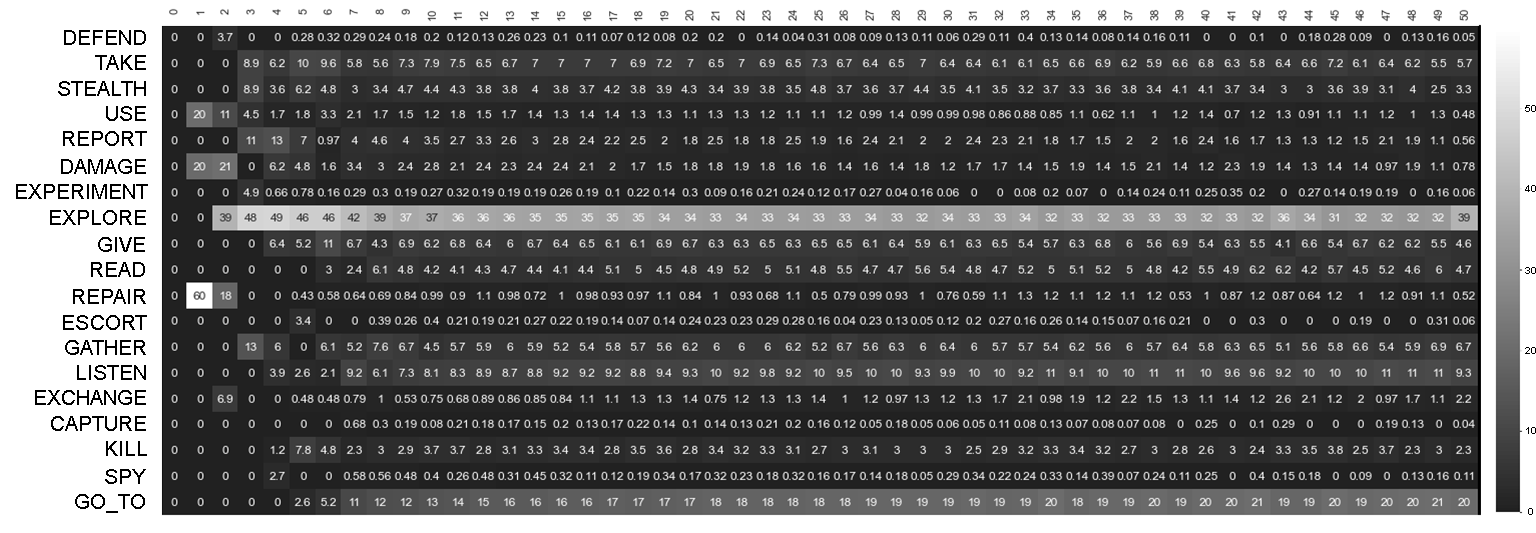
\includegraphics[width=1\textwidth]{included-papers-tex/paper-8/figures/perLengthExperiment-an.png}
        \caption{Chance (in \%) for every quest action (row) to appear in a quest of a given length (column).}
        \label{figs:evaluation:length}
    \end{subfigure} \hfill% \
    %  \captionsetup[subfigure]{width=0.9\textwidth}
    \begin{subfigure}[t]{0.9\textwidth}
        \centering
         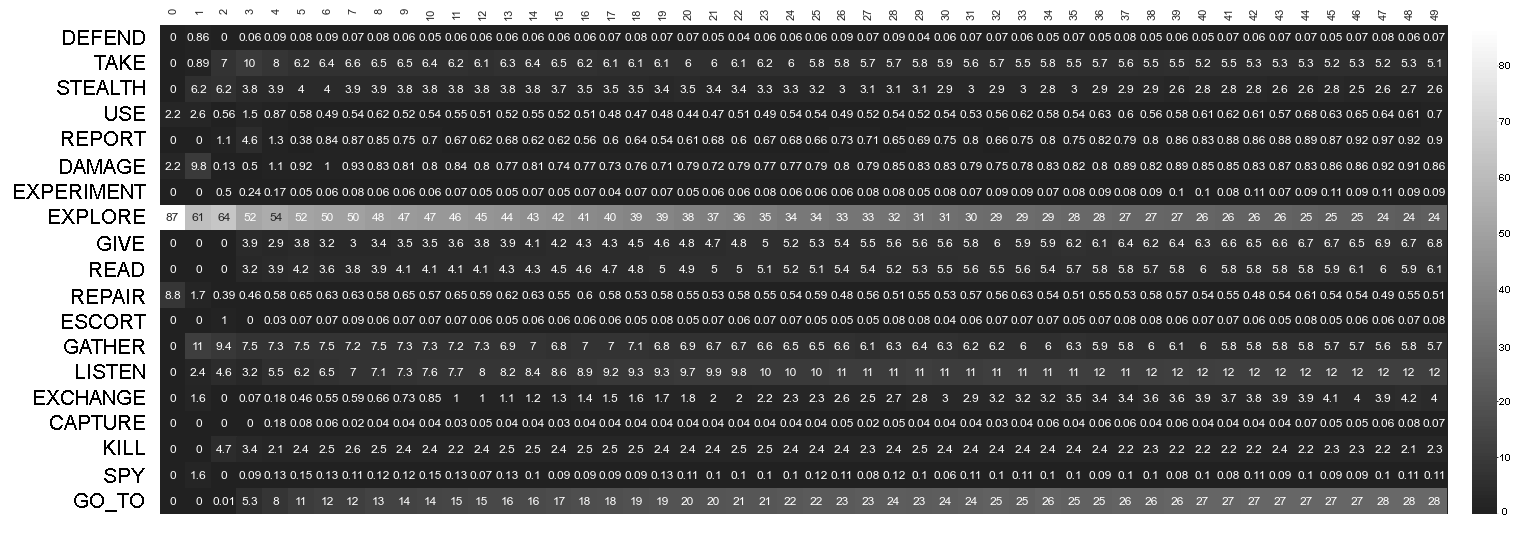
\includegraphics[width=1\textwidth]{included-papers-tex/paper-8/figures/perStepsExperiment-an.png}
        \caption{Chance (in \%) for every action (row) to appear at the Nth step of a quest (column), regardless its length.}
        \label{figs:evaluation:steps}
    \end{subfigure}
    \caption{Results from the Expressive Range Analysis}
    \label{figs:Experiments}
\end{figure*}

\begin{figure}[]
    \centering
    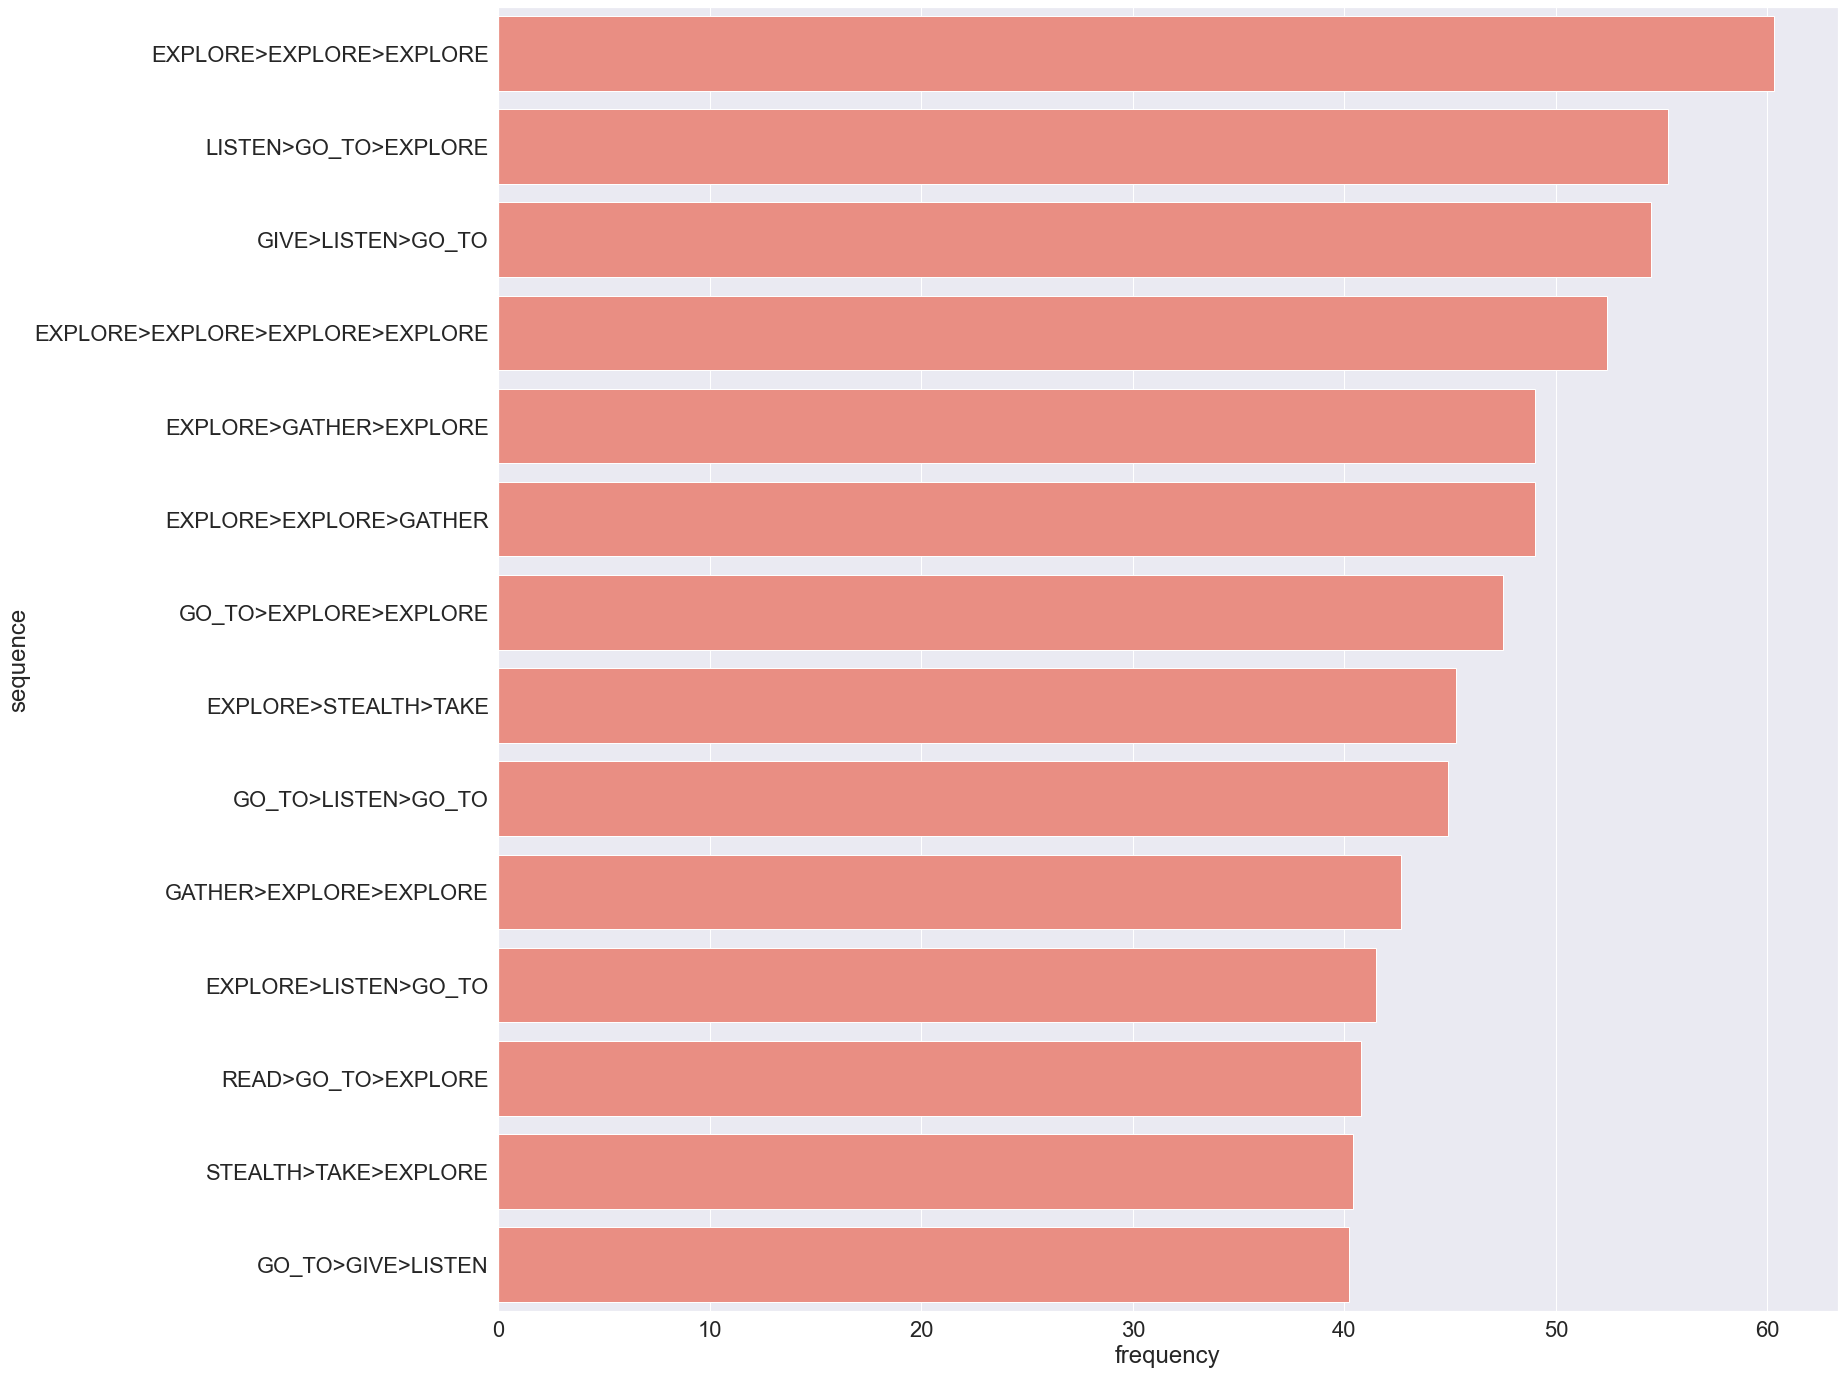
\includegraphics[width=0.9\textwidth]{included-papers-tex/paper-8/figures/CommonSubsequence-GSP.png}
    \caption{Most commonly generated subsequences, with a minimum size of 3.}
    \label{figs:evaluation:CommonSequence}
\end{figure}



\subsubsection{User Study}



% The evaluation of the artefacts usability and functionality was evaluated through a small user study. When evaluating PCG systems, Shaker et. al argues that when making a PCG system, “we are also creating a large amount of content for players to experience, thus it is important to be able to evaluate how successful the generator is according to players who interact with the content”~\citepeighth{p8shaker_procedural_2016}. In our case, EDD is a development tool for designers and not for actual players, but we argue that the actor interacting with the system, in our case, the designer, still is the interactive actor and thus we have decided to do an evaluation with actual potential users of the artefact. An additional advantage of conducting a user study is that it evaluates the aspects that cannot be objectively measured, such as aesthetics and playing experience~\citepeighth{p8Yannakakis2018}. In addition, previous studies on mixed-initiative systems have been conducted through a user study, such as the first version of  EDD[35], its second follow-up study [36] and Sentient Sketchbook [24]. 

% \subsubsection{Results}

Six participants tested our tool following three pre-designed tasks and questionnaires to evaluate Questgram's usability, functionality, and usability. They were all given a document describing the study's purpose and aim, a brief introduction to EDD, and the interview overview. The users were then asked to complete three tasks that covered the tool's functionality and different approaches to creating quests. The tasks were to 1) manually create a quest, 2) automatically create a quest, and 3) create a quest through mixed-initiative. They were also asked to create a dungeon that suited their preferences and objectives before creating quests. The questionnaire consisted of 17 closed-ended questions, and the rest were open-ended. The interview began with a questionnaire with six questions about the users' background and experience within game development and finish with questions about their experience and opinions on the tool. Both the questionnaire and interview followed guidelines described by Oates~\citepeighth{p833-ResearchingInfoSystems}.  

The participants were selected through convenience sampling and were game developers working in game and level design (2) and game development alumni (4), without any experience with EDD or mixed-initiative tools. Five out of six have played dungeon/adventure games and have developed some game with quests and missions, while only two out of six have developed dungeon style games.

\paragraph{Manual Quest Creation}

Participants reported that the tool was easy to use, clear, intuitive, and while simple and basic, it had enough building blocks for them to create their objective quest. Positive feedback was also given regarding the UI, integration with the rest of EDD functionalities, clarity of the quest action concerning the quest, and making the tool overall more interesting. However, some participants expressed confusion when quest sequences became too large as they would have preferred to separate the quests into sections or subquests. Another concern expressed was the inability to change the order of already created quests without redoing the whole quest sequence.

\paragraph{Automatic Quest Creation}

Some participants reported that the system showed potential and a good addition to the manual creation, especially for the creation of side quests such as how similar systems work in \emph{Skyrim}, and for learning how to use the tool as some kind of tutorial. Nevertheless, most participants remarked the system as random and illogical regarding random tile picks connected with quest actions as the system picked farther away NPC and targets with no purpose. In addition, participants felt that a system like this complicated the creation and took the freedom of creating their world and ideas. 

\paragraph{Mixed-Initiative Quest Creation}

The participants described the system as helpful and useful; pointing out that the main advantages and potentials were related to when they reached an inspiration blockage as the designer could get inspired by the suggestions; to allow designers to focus on key parts of a quest sequence, and the speed gained to create quests "in just a matter of moments." While most feedback was positive, there were still concerns among participants regarding the system's cohesiveness as it could feel hard to make the suggestions cohesive with what the participant had in mind. Nevertheless, a majority of the participants experienced that both the manual and automatic complemented each other.

\paragraph{Automatic Suggestions}

Participants generally described the automatic suggestions as useful to gain inspiration, keep the quest creation diverse, and learn what could be created, rather than useful to replace or add to their work. For instance, one participant said that "[the system] suggested to capture a monster which had thought about killing. The "capture" option might be more interesting and might have been an option I had otherwise overlooked." Similarly, another participant pointed out that the automatic suggestions "... were useful in getting inspiration for quests, and to learn the program and what kinds of quests I was actually able to make." Usually, designers have a predetermined idea on how they would like the narrative to unfold. However, based on the responses we received, the system gave a different perspective to the users on what they could create or how they could continue a quest, which makes the tool useful for brainstorming quest design similar to tools such as Questbrowser~\citepeighth{p8Sullivan2009-questbrowser}, albeit constrained to the possible quest actions.

Still, participants preferred to use the system as inspiration rather than effectively incorporating changes to the quests. This was mainly due to the suggestion not feeling cohesive enough with what participants created until then, and the random tiles picked for the quest action. For instance, receiving a "GO TO" suggestion to a random tile on the opposite side of the level and not near the player or the previous quest action.


% However, most participants described the automatic suggestions as inspiring rather than useful to replace or add to their work. 
% It worked well for looking though the options and deciding which would be best to use or to find possibilities that I had not previously considered. They were not very good at applying directly. Say that it suggested to capture a monster which had thought about killing. The "capture" option might be more interesting and might have been an option I had otherwise overlooked. Still not great for suggestions to apply directly but a good way to look at your options.

% This would have good potential for making the designers be able to focus better on the parts that were important in a quest, and let the computer make up the steps inbetween. I think generally it would make a bit more sense for a player to set a start and a goal for a level, then have the computer generate bits in between those.

% The mixed creation was helpfull for me since i like to do it all myself but when i reaced a inspirationblock the automatic came in and helped move it along. The automatic suggestions changed dynamicly with whatever i added to my own questline.

% I liked the possibility to use a suggestion when I wanted inspiration or ran out of ideas myself. For me personally I don't think it's a more efficient way to create quests for the same reason that he suggestions often don't work with the quests that has already been chosen- or that it's just faster to do it manually. So the final thought is that I think that it's a nice thing to have, but I would probably use manual creation more.

% Yes, it was useful. It gives you some ideas to what you can do. You can build further on those ideas. Though it could have been a bit more.

% The automatic suggestions, for me personally, were useful in getting inspiration for quests, and to learn the program and what kinds of quests I was actually able to make. I personally didn't find it useful in speeding up or making the creation more efficient, but it feels like a nice tool to have if you get stuck or want some new ideas.

\paragraph{Quest Actions}

Quest actions and their goals were perceived as easy to understand and suitable for the type of game they were creating, except for "experiment," "stealth," and "spy," since they felt ambiguous and not clear for some participants. Fulfilling some quest actions' prerequisites was somewhat obscure, and some participants needed to go through trial and error to gain access to the quest action. However, once they fulfilled the prerequisites, it was clear and made sense in the context.

\paragraph{Usability}

All participants described the tool as a useful addition for game developers when developing dungeon games but with different arguments and situations on when it would be useful. For instance, to create mundane quests in games with a grinding flow such as \emph{Diablo}, to fast-prototype ideas and systems to give insights into what it might be possible and what might work, and to complement the creation of content and quest-design. Some participants expressed that making the game playable is a must to get the full benefit from the tool.

\paragraph{Creativity}

Most of the participants reported that they experienced increased creativity when using mixed-initiative creation. The participants described that it helped when they got stuck, and it showed different alternatives and routes they did not previously consider. Further, one participant explained that they could make more creative decisions and not "staying safe" and adding "extra steps" without any effort. For instance, using a spy before a kill, thus prolonging the sequence by an extra action. Two participants highlighted that while they did not experience increased creativity, they saw the tool as useful when no new ideas are there given the possible "out of the box" suggestions.

\paragraph{Overall Experience and Missing Features}

Some participants expressed that the tool was useful for someone in the gaming community, but it would be hard to grasp for someone unfamiliar with the concept. Further responses were that it was simple to work with, felt scalable, and the software's recommendation felt useful when designing a quest. Additional response from one participant, who, despite having no prior experience in either creating or playing dungeon games, said it was a fun introduction to the genre and that it was easy to learn and understand. Further, they explained that the simple workflow inspired them to continue creating. In addition, further responses were that the software was quick, feature-rich, simple to use, and got their creativity flowing.

In general, the participants expressed that more interaction with the quest sequence itself, such as changing the order of subsequences, adding quest actions in arbitrary parts, having separate quests, or knowing which quests were manually and automatically, would improve the system considerably. 

\subsubsection{User Study Discussion}

Since we use the work by Doran and Parberry~\citepeighth{p8Doran2011-questsMMORPGs} as a base for the quest generation, this research indirectly tests their quest patterns and their applicability into a mixed-initiative tool. We leveraged on these quest patterns similar as others have on quest patterns~\citepeighth{p8Trenton2010-questpatterns,p8Smith2011-situatingQuests}, and how EDD leverages on level design patterns for the level generation~\citepeighth{p8Baldwin2017,p8alvarez2019empowering}. The use of quest patterns greatly improves the communication with the designers as they can use concepts they feel comfortable with and relate better to the content they create. All of our participants confirmed the previous statement by pointing out how the tool was straightforward, easy to understand with quests actions to be found in any other game type, and easy to use even if they had never used a mixed-initiative tool.
% We leveraged on the quest patterns defined by Doran and Parberry~\citepeighth{p8Doran2011-questsMMORPGs} similarly to how EDD leverages on level design patterns for the level generation facet~\citepeighth{p8Baldwin2017,alvarez2019empowering}.

% Leveraging on game design patterns is not new~\citepeighth{p8Bjork2004-GameDesignPatterns} and similar conclusions have been presented before~\citepeighth{p814-Dahlskog2015-patternsDungeonsGens,Smith2011-situatingQuests,Trenton2010-questpatterns,Baldwin2017,Alvarez2018}; thus, our user study confirms.

Furthermore, while relevant, the suggestions by the system felt impractical mainly and according to participants because the system randomly assigned tiles for the suggested quest action, which limited the tool's perceived usability. Another reason is the use of abstract quest actions. On the one hand, this allows us to disconnect the system from specific implementations and gameplay functionalities of the quests, creating and representing a more generic system. On the other hand, this resulted in a lack of thematic and concrete elements such as NPC roles or defined plot lines and plot elements to follow. These make it harder for designers to contextualize their creations and why the system recommends specific quest actions. %Some preliminary study was done 

%On the other hand, this lack of thematic and concrete elements such as NPC roles, and defined plot lines and elements to follow, makes it harder for designers to contextualize their creations and what or why the system recommends certain quest actions.

Nevertheless, the system was helpful for creativity support and design aid as the suggestions were used as an inspiration to what was possible and what to do next rather than using the actual suggestion. Participants only applied suggestions when the next step felt mundane, and the system suggested a logical position. Leveraging on the human designer for deciding location, while the system provides the quest actions that would follow a more typical quest based on the quest patterns would probably compose a better collaboration. 

%Likewise, this also shows the need for exploring other fundamental and useful ways to establish human-AI collaboration, specifically MI-CC tools that effectively enables the proactive collaboration and creation. Some preliminary study showed that when adding NPC roles and adapting Questgram to it, helps the users contextualize and create quests more alike common quests in RPG. Yet, users used even less the suggested actions as it was seem as "help for novices," rather than a way to create quests between both. This points towards the need to explore other fundamental and more useful ways to establish MI-CC workflows where systems can adapt and create ~\citepeighth{p8Zhu2018-XAIDesignersMICC}. , but reducing even more the use of the suggested actions, 

%Furthermore, while relevant, the suggestions by the system felt impractical because the system randomly assigned tiles for the suggested quest action. This limited the tool's perceived usability as participants used the suggestions more as an inspiration to what was possible and what to do next rather than using the actual suggestion. Participants only used suggestions when the next step felt mundane, and the system suggested a logical position. Leveraging on the human designer for deciding location, while the system provides the quest actions that would follow a more typical quest based on the quest patterns would compose a better collaboration.

%Nevertheless, it is important to point out that we are using and suggesting abstract actions represented in a generic way to disconnect the system from specific implementations. On the one hand, this allows us to to disconnect the system from specific implementations and gameplay functionalities of the quests. On the other hand, this lack of thematic and concrete elements such as NPC roles, defined plot lines 

%While our tool is helpful for creativity support

Some feature suggestions such as separating quests or reordering the quest sequence would have improved the user experience considerably, as after manually placing just a few quest actions, the quest became harder to approach. Even if the system was tested to generate 50 quest actions as explained in section~\ref{sec:quantExp}, this might be impractical for human designers. An interesting suggestion was to use color tags or similar to understand which agent (Human or machine) created the quest. Then, designers could also use this as a way to understand decisions made by the system and for the system to create a model of the current designer's quests. This could also be used for a collaborative tool where several designers interact with each other and a centralized system; for a more crowdsourced approach such as the one proposed by Charity et al.~\citepeighth{p8charity2020baba}.

%\subsubsection{General Discussion}



%My takeaway from the paper is that support at the level of abstract actions does not provide enough designer support. Designers rarely make use of the suggested actions, but instead use them for inspiration. Further, human designers generally didn’t like the fully automatically generated quests, but instead found them random and illogical. This is ascribed to the random floor tile placement, but I wonder, even with smarter floor tile placement, if the generated quests would still feel unmotivated due to the lack of thematic elements. I would like to hear a discussion from the authors about their conclusions regarding the limits of abstract action grammars, on their own, as design aids. 

%In quests generated by this system, the player spends most of their time just moving around between locations. How can one make all this movement feel motivated for both players and designers? It seems to me that this requires thematic and plot elements. 

%-	In summary, the conclusion I’m drawing from all this as a reader is the somewhat negative result that a grammar of abstract quest actions, on their own, does not provide sufficient quest design support, because of the lack of integration with gameplay, thematic and story elements.  

%R2’s idea is based on the notion that because “[d]esigners rarely make use of the suggested actions,” and found the “fully automatically generated quests… random and illogical,” one way of interpreting these results is as “the somewhat negative result.” That is “a grammar of abstract quest actions, on their own, does not provide sufficient quest design (R2).” From my reading of R2’s review, they are drawing on the often noticed but swept-under-the-rug finding that mixed-initiative tools are most helpful as inspirational aides. But I wanted to point out to the authors that they have a chance here to inspire future creators of mixed-initiative tools by speculating on the limitations of a “grammar of abstract quest actions on their own.” Regardless it would be an interesting avenue for future work/studies.

%-	Another question I had was how the quest actions are supported in the gameplay code. For example, to me the spy action involves watching an NPC to learn some information, while not being observed by the NPC. So, from a gameplay perspective, I could imagine an implementation where the player has to stay outside of the view cone of an NPC, while the NPC performs actions that result in the player learning something. But from the prerequisite table, it sounds like all that is needed is an NPC that the player can move to . 

%Do a bit more discussion on problems with abstract quest design and those things. and the benefits of using these quest design 

% Some feature suggestions, while straightforward such as separating quests or reordering the quest sequence were not implemented 



% \begin{enumerate}
%     \item Manually creating a quest sequence
%     \item Automatically generating a quest sequence
% \end{enumerate}